% Chapter 4

\chapter[Implementation and on-sky testing]{\setstretch{1}Implementation and on-sky testing} % Main chapter title


%\epigraph{\setstretch{1}\small\itshape Ever tried. Ever failed. No matter. \\ Try again. Fail again. Fail better.}{S. Beckett, \textit{Worstward Ho!}}

\section{Key pre-flight procedures}
\subsection{Inertia measurement}
While CAD models allowed to us to estimate the moment of inertia of the payload, this is only an approximation. For testing and for launch, the payload will be different than the model we have: we will either miss some components because they are not yet installed, or have additional components such as the ballasts, the crush pads, or the weights that are used to balance the payload.

We use a simple procedure to estimate the moment of inertia about $\gyroVec{z}_\gyro$ of the payload while hanging from a crane. For this purpose, we command the CCMG to input a torque to the payload by moving the gimbal at a constant velocity. According to Eq.~\ref{eq:CCMGTorque}, $\ccmgtorque =  20.8\times \dot{\theta}\cos\theta$. According to conservation of angular momentum, the rate of change of the total angular momentum about $\vectors{z}_\gyro$ is $\inertia_\vectors{z}\dot{\gyroVec_\vectors{z}} = \ccmgtorque = 20.8\times \dot{\theta}\cos\theta$.

We measure the inertia $\inertia_\vectors{z}$ by averaging measurements of the angular acceleration $\dot{\gyroVec_\vectors{z}}$, divided by the instantaneous input torque, which is numerically more stable than averaging its inverse since the accelerations, expressed in \si{\radian\per\second} are typically very small. A measure of the inertia is then the inverse of this average. By repeating the measurement over multiple accelerations and deceleration cycles, we can also obtain an uncertainty to this estimate.

[PUT HERE A TABLE WITH MEASURED INERTIA AND UNCERTAINTIES]

\subsection{Sensor alignment and calibration}
While the intrinsic noise of our sensors has been characterized in Section~\ref{subsec:gyros}, it is important to test them while mounted to the payload, align their axes to the other reference frames, and study their spectral energy distribution. Mounting the gyroscopes in a 3-dimensional mount on the truss will inevitably lead to alignment errors and the contribution of new vibration frequencies present in the structure and excited by the moving parts on the payload.


\subsubsection{Gyroscope spectral analysis in flight configuration}

While the payload is on the ground, without wheels;

While the payload is hanging, without wheels

While the payload is hanging, with wheels on;

\subsubsection{Orthogonalization of gyroscope mount}
\label{ap:gyroOrth}
\subsubsection{Alignment of gyroscope mount to star camera mounts}

BETTII will have two flight star cameras for redundancy. It is important to understand the transformation between the gyroscope reference frame and the two star camera reference frames to minimize the propagation errors within the Kalman filter. 

A first transformation matrix can be estimated roughly by assuming that the star camera is in the ($\vectors{x}_\gyro$,$\vectors{z}_\gyro$) plane. The elevation of the star camera, nominally around \SI{45}{\degree}, can be estimated if $\vectors{z}$ is assumed to be aligned with the gravity vector while the payload is sitting on the ground, which is a good approximation. By taking some star camera measurements, solving the fields, and converting these fields to a local azimuth and elevation (using the time at which the frames were taken and the geographical location), the elevation can be estimated, which corresponds to the angle of the line of sight vector of the star camera with respect to the horizontal plane. This gives us a first estimate of our star camera-to-gyroscope reference frame rotation, but is not very precise given our assumptions. This rotation is critical during the update phase of the Kalman filter when combining the star camera measurement with the propagated estimate.

But if this matrix is slightly off, the Kalman filter will attribute the difference between estimated position and measured position as an additive bias error in the gyroscope velocity measurement, which should converge to a steady-state value after a few tens of star camera measurements, depending on the Kalman filter gains. The filter then uses this additive bias to reconstruct an estimated velocity at each time step. Admittedly, this value of the bias also contains the value of the real gyroscope bias - but we anticipate  this bias value to be very small compared to the potential effects of misalignments.

Our procedure involves calculating the quaternion representing the rotation from the steady-state estimated angular velocity vector, and the measured, orthogonalized angular velocity vector. While sitting on the ground, this corresponds to measuring the Earth's angular velocity. This uses the mathematical technique that we derived in Appendix~\ref{ap:rotBetweenTwoVec}. Each star camera measurement shall be further rotated by this quaternion to ensure that it is properly expressed in the gyroscope reference frame. 

Below, we summarize the steps to properly align the gyroscopes to the star camera:
\begin{enumerate}
 \item Orthogonalize the gyroscope mount according to Appendix~\ref{ap:gyroOrth}, and find $M_\textrm{orth}$. This now gives a velocity vector in an orthogonal gyro reference frame, $\gyroVec_\gyro$ = $M_\textrm{orth}\gyroVec_\gyro^\textrm{meas}$. 
 \item While the truss is sitting horizontal on the ground, calculate the elevation of the star camera by converting solutions to the local East-North-Up reference frame, using the sidereal time and the geographical latitude. This gives a matrix $M_\textrm{coarse}$  or a quaternion $\quat{q}_\textrm{coarse}$ representing the transformation from the star camera reference frame to the gyroscope reference frame.
\item Still while sitting on the ground, use $M_\textrm{coarse}$ or $\quat{q}_\textrm{coarse}$ in the flight Kalman filter to estimate the gyro bias vector. Record the steady-state value of the estimated velocity vector.
 \item Calculate the transformation between the estimated and measured angular velocity vector, this is a matrix $M_\textrm{fine}$ or a quaternion $\quat{q}_\textrm{fine}$.
 \item For each star camera reference frame solution, rotate the solution $\quat{q}_\textrm{fine}\quat{q}_\textrm{coarse}$.
 \item Use this new matrix in the flight Kalman filter to make sure the estimated biases are close to zero. 
 \end{enumerate} 
\subsection{Star camera}
\subsubsection{Software tuning}

\begin{landscape}
\begin{figure}[!ht]
	\centering
	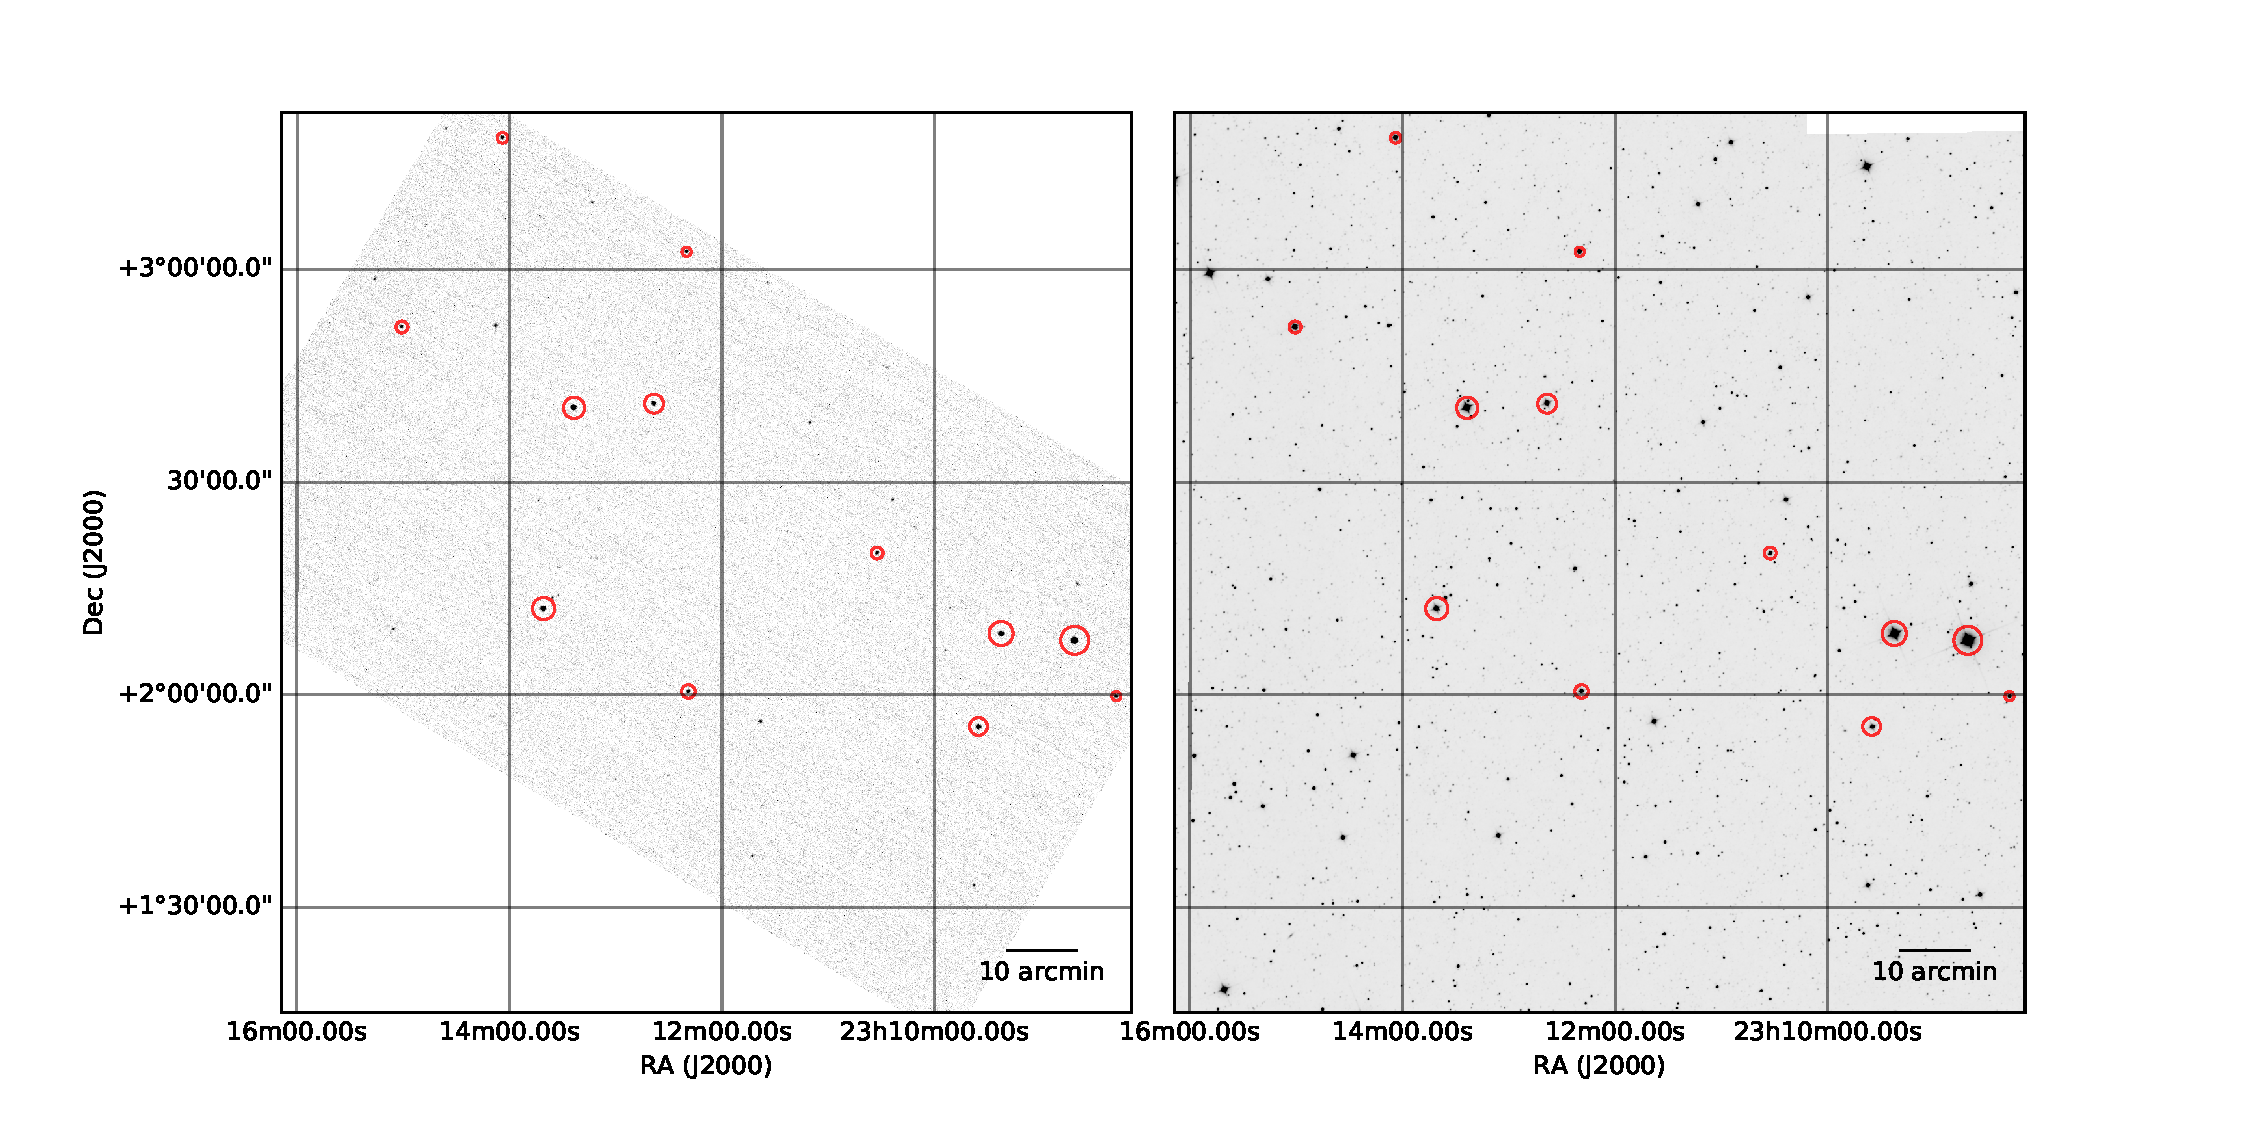
\includegraphics[width=1.5\textwidth]{Figures/starcam_images.pdf}
	\caption[Star camera example WISE]{\textit{Left}: Example of a background-subtracted star camera image with identified $>5\sigma$ sources circled in red. The orientation of the image on the celestial sphere is the one provided by BETTII's embedded star camera solver. This image corresponds to a field in the Scorpius constellation. \textit{Right}: WISE \SI{3.4}{\um} mosaic from the online archive, centered on the same location. This image is composed of 9 individual WISE images that we patched into a mosaic using the \textit{Montage}[CITE] software package.}
	\label{fig:starcamexample}
    \end{figure}
\end{landscape}
\begin{landscape}
\begin{figure}[!ht]
	\centering
	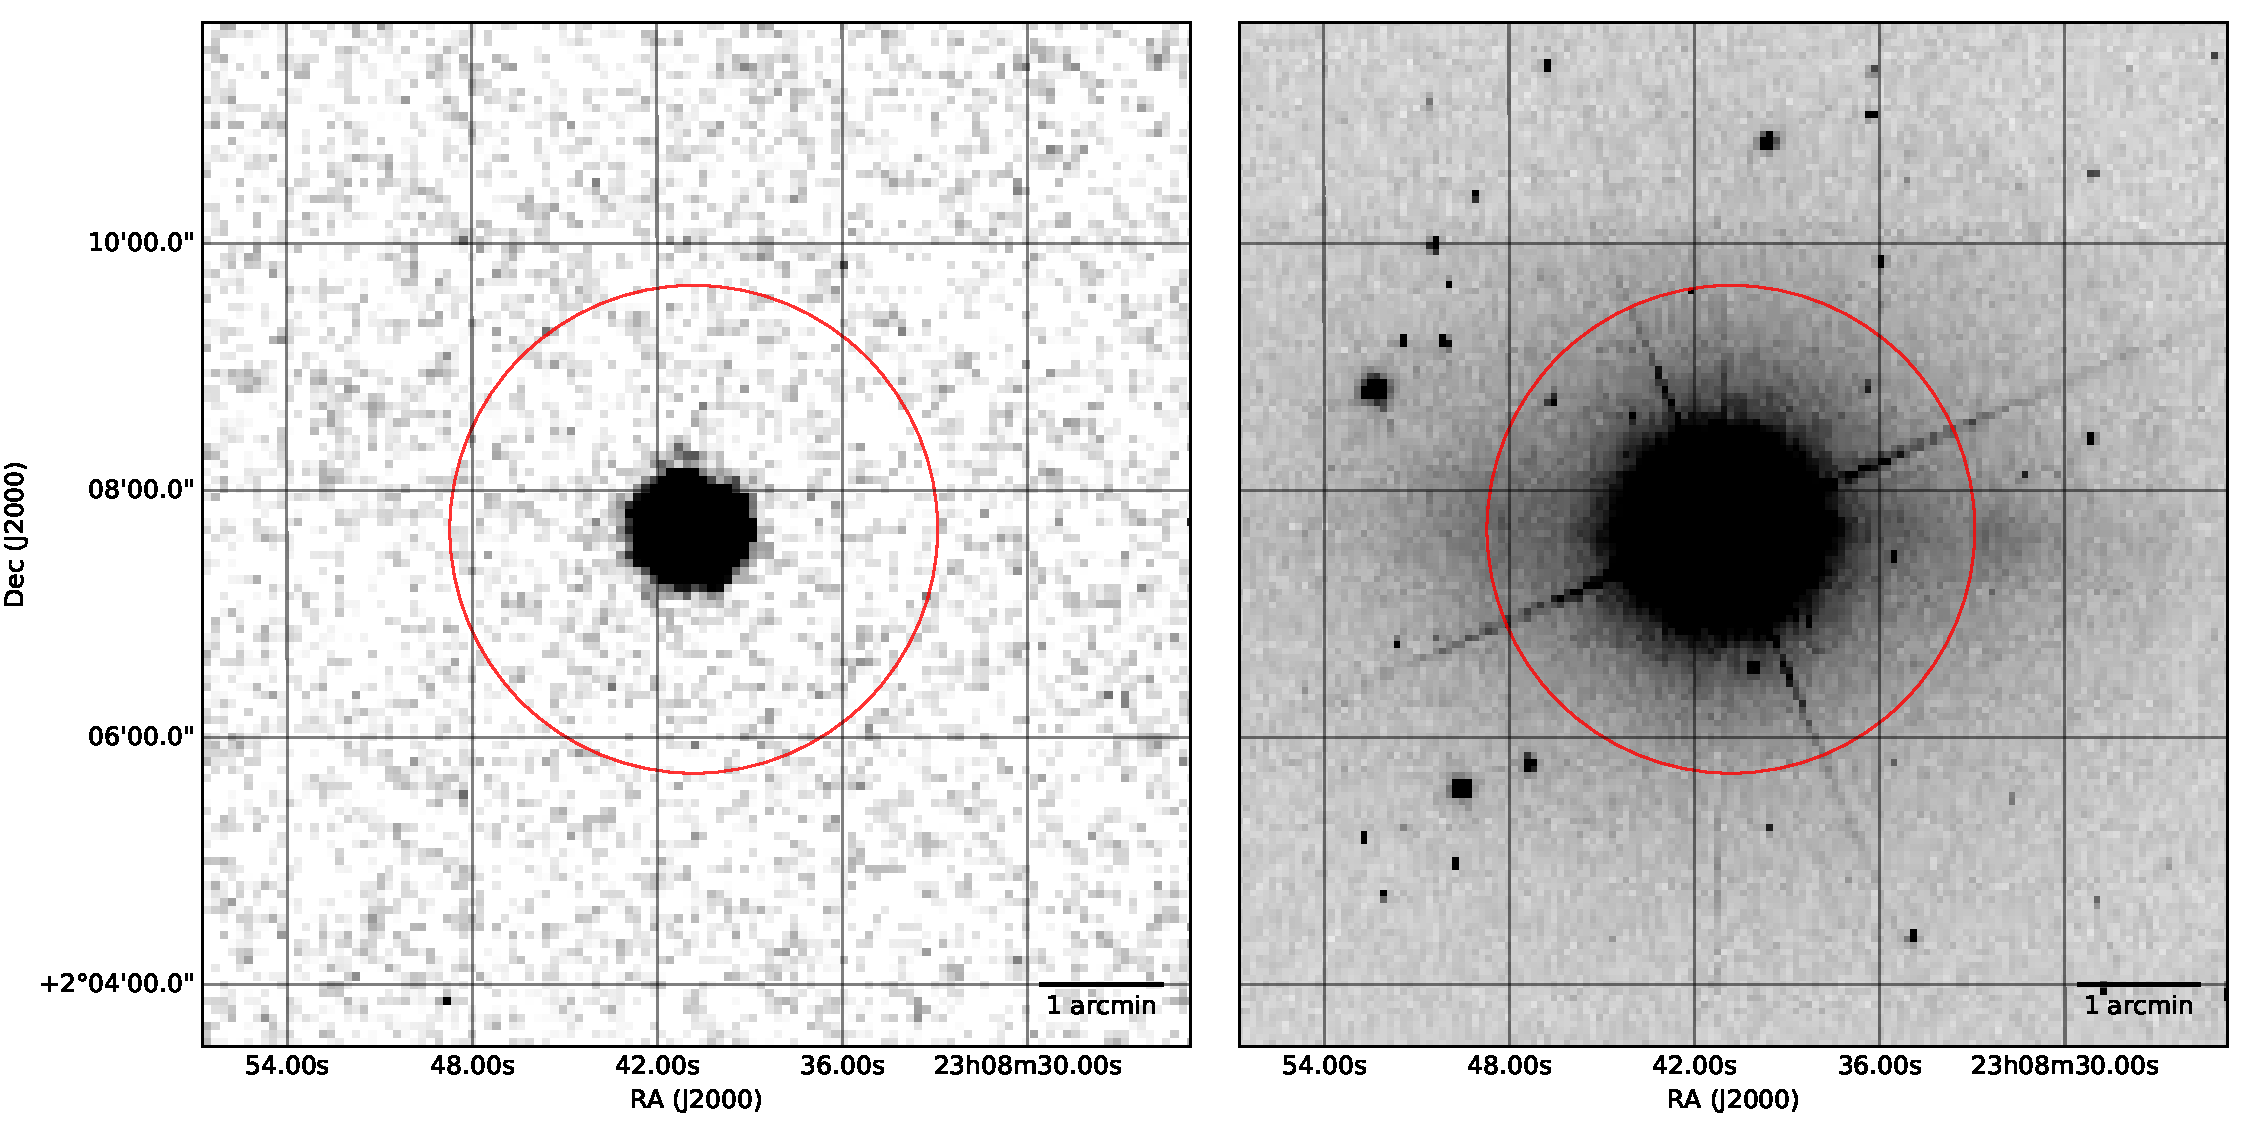
\includegraphics[width=1.5\textwidth]{Figures/starcam_SDSSr_zoom.pdf}
	\caption[Star camera individual star]{\textit{Left}: Snapshot of a bright star seen within the background-subtracted star camera frame. \textit{Right}: Snapshot taken at the same location from the WISE \SI{3.4}{\um} archive.}
	\label{fig:starcamzoom}
    \end{figure}
\end{landscape}

Discuss about tuning, catalog, filters, etc

Table with the star camera parameters

Show mean deviation of star camera image with optimized parameters;
show time, statistics, etc.

\subsubsection{Calibration}

\section{Test setups and limitations}
\subsection{Talk about the way we test in the high bay, etc}
\subsection{List of test setups: gyro only, gyro+star camera, gyro+star camera+tip/tilts with CCD cameras, gyro+star camera with H1RG;}
\subsection{Explain the communication/data recording approach}

\subsection{Autofocus algorithm and performance}

\section{Estimator implementation}
\subsection{Gyro attitude estimator}
\documentclass{standalone}
\usepackage{tikz}
\usetikzlibrary{shapes,arrows}

\begin{document}
\tikzstyle{block} = [draw, fill=black!20, rectangle, 
    minimum height=3em, minimum width=6em,align=center]
\tikzstyle{input} = [node distance=1cm]
\tikzstyle{output} = [node distance=1cm]
\newpage
\begin{tikzpicture}[auto, >=latex',scale=0.8, every node/.style={transform shape}]
\linespread{1}


% Inputs
\node [input,name=measuredVelocity,shift={(2cm,0cm)}] {$\gyroVec^{\textrm{meas}}_k$};
\node [input,above of=measuredVelocity,name=bias] {$\EstBias_{k|k-N}$};
\node [input,above of=bias,name=attitude,node distance=1cm] {$\EstAttitude_{k-1|k-N}$};
\node [input,above of=measuredVelocity,name=covariance,node distance=3cm] {$\noiseCovMat_k$};
\node [input,below of=measuredVelocity,name=propagation matrices,node distance=4cm] {$\A_{k-1},\B_{k-1},\C_{k-1}$};

% line break
\node [input,name=line break left,above of=covariance,node distance=2cm] {};
\node [input,name=line break left2,below of=line break left,node distance=0.5cm,right] {\large \textbf{Kalman Filter: Prediction}};
\node [input,name=line break right,right of=line break left,node distance=15cm] {\large { }};
\draw[dashed] ([xshift=-1cm]line break left.north west) -- (line break right.north east);


% blocks
\node [block, right of=measuredVelocity,node distance=3cm] (estimate velocity) {Estimate \\ Velocity};
\node [block, right of=estimate velocity,node distance=4cm] (predict attitude) {Predict \\ Attitude};
\node [block, below of=predict attitude,node distance=2cm] (state transition) {State \\ transition};
\node [block, right of=state transition,node distance=4cm] (estimate covariance) {Estimate \\ covariance};
\node [block, below of=estimate covariance,node distance=2cm] (update propagation matrices) {Propagate \\ matrices};

% outputs
\node [output,right of=predict attitude,node distance=3cm,name=estattitude]{};
\node [output,right of=estimate covariance,node distance=3cm,name=estcovariance]{};
\node [output,right of=update propagation matrices,node distance=3cm,name=propmat]{};

% arrows
\draw[->] (bias.east) -| (estimate velocity.north);
\draw[->] (measuredVelocity.east) -- (estimate velocity.west);

\node[name=mid,right of=estimate velocity,node distance=2cm,draw,fill,minimum size=3pt,circle]{};
\node[above] at (mid){$\EstGyroVec_{k|k-N}$};
\draw[->] (estimate velocity.east) -- (mid) -- (predict attitude.west);
\draw[->] (attitude.east) -| (predict attitude.north);
\draw[->] (mid) |- (state transition.west) ;
\node[name=mid,right of=state transition,node distance=2cm,draw,fill,minimum size=3pt,circle]{};
\node[above] at (mid){$\StateTransitionMat_k$};
\draw[->] (state transition.east) -- (mid) -- (estimate covariance.west) ;
\node[name=mid2,below of=mid,node distance=1cm,outer sep=0cm,inner sep=0cm]{};
\draw[-] (mid) --  (mid2.north) ;
\draw[->] (mid2.north) -|  (update propagation matrices.north) ;

\node[name=mid,right of=estimate covariance,node distance=3cm]{};
\node[above] at (mid){$\stateCovMat_{k|k-N}$};
\draw[->] (estimate covariance.east) -- (estcovariance) ;
\draw[->] (covariance.east) -| (estimate covariance.north) ;

\node[name=mid,right of=predict attitude,node distance=3cm]{};
\node[above] at (mid){$\EstAttitude_{k|k-N}$};
\draw[->] (predict attitude.east) -- (mid);

\draw[->] (propagation matrices.east) -- (update propagation matrices.west);
\draw[->] (update propagation matrices.east) -- (propmat);
\node[name=mid,right of=update propagation matrices,node distance=3cm]{};
\node[above] at (mid){$\A_{k},\B_{k},\C_{k}$};


% Kalman Update
% line break
\node [input,name=line break left,below of=propagation matrices,node distance=1.5cm] {};
\node [input,name=line break left2,below of=line break left,node distance=0.5cm,right] {\large \textbf{Kalman Filter: Update}};
\node [input,name=line break right,right of=line break left,node distance=15cm] {\large { }};
\draw[dashed] ([xshift=-1cm]line break left.north west) -- (line break right.north east);

% Inputs
\node [input,name=measured attitude,below of=line break left,node distance=3cm] {$\Attitude^\textrm{meas}_{\starcam}$};
\node [input,name=final matrices,above of=measured attitude,node distance=1cm] {$\A_{k},\B_{k},\C_{k}$};
\node [input,name=covmat,below of=measured attitude,node distance=6cm] {$\stateCovMat_{k|k-N}$};
\node [input,name=meascovmat,below of=measured attitude,node distance=2cm] {$\measCovMat_{k}$};

% blocks
\node [block, right of=measured attitude,node distance=3cm] (propagate attitude) {Rotate \& \\ Propagate};
\node [block, below of=propagate attitude,node distance=2cm] (innovation) {Innovation};
\node [block, below of=innovation,node distance=2cm] (innovation covariance) {Innovation \\ covariance};
\node [block, below of=innovation covariance,node distance=2cm] (kalman gain) {Kalman \\ gain};
\node [block, right of=kalman gain,node distance=4cm] (calculate error) {Calculate \\ error};
\node [block, right of=calculate error,node distance=4cm] (update bias) {Update \\ bias};
\node [block, below of=update bias,node distance=2cm] (update attitude) {Update \\ attitude};
\node [block, above of=update bias,shift={(3cm,1cm)}] (update velocity) {Update \\ velocity};
\node [block, below of=update attitude,node distance=2cm] (update covariance) {Update \\ covariance};

% arrows
\draw[->] (measured attitude) -- (propagate attitude);
\draw[->] (final matrices) -| (propagate attitude);
\draw[->] (propagate attitude.south) -- (innovation.north);
\draw[->] (innovation covariance.south) -| (kalman gain.north);
\draw[->] (covmat.east) -- (kalman gain.west);
\draw[->] (covmat.north) |- (innovation covariance.west);
\draw[->] (meascovmat.east) -- (innovation.west);
\draw[->] (covmat.south) |- (update covariance.190);

% intermediary nodes
\node[name=mid,right of=kalman gain,node distance=2cm,draw,fill,minimum size=3pt,circle]{};
\node[above] at (mid){$\KalmanGain_{k}$};
\draw[->] (kalman gain.east) -- (mid) -- (calculate error.west);
\draw[->] (mid) |- (update covariance.165);

\node[name=mid,below of=propagate attitude,node distance=1cm]{};
\node[left] at (mid){$\Attitude^{\textrm{meas}}_{k}$};


\node[name=mid,below of=innovation,node distance=1cm,draw,fill,minimum size=3pt,circle]{};
\node[left] at (mid){$\zMeasurement_{k}$};
\draw[->] (mid) -| (calculate error.north);
\draw[->] (innovation.south) -- (mid) -- (innovation covariance.north);

\node[name=mid,below of=innovation covariance,node distance=1cm]{};
\node[left] at (mid){$\measErrCovMat_{k}$};


\node[name=mid,right of=calculate error,node distance=2cm,draw,fill,minimum size=3pt,circle]{};
\node[above] at (mid){$\ErrorState_{k|k}$};
\draw[->] (calculate error.east) -- (mid) -- (update bias.west);

\node [input,name=bias estimate,above of=mid,shift={(1cm,0cm)}] {$\EstBias_{k|k-N}$};
\draw[->] (bias estimate) -| (update bias.north);

\node [input,name=attitude estimate,below of=bias estimate,node distance=2cm] {$\EstAttitude_{k|k-N}$};
\draw[->] (attitude estimate) -| (update attitude.north);


\node [input,name=velocity estimate,above of=bias estimate,node distance=2cm] {$\EstGyroVec_{k|k-N}$};
\draw[->] (velocity estimate) -| (update velocity.north);
\draw[->] (mid) |- (update attitude.west);

\node [output,name=velocity,right of=update velocity,node distance=2cm]{}; \node [output,right of=update velocity,node distance=2cm,above] {$\EstGyroVec_{k|k}$};
\draw[->] (update velocity.east) -- (velocity);

% outputs
\node [output,name=mid,right of=update bias,node distance=3cm,draw,fill,minimum size=3pt,circle] {};
\draw[->] (update bias.east) -- (mid);
\draw[->] (mid) -- (update velocity.south);
\node [output,name=bias,right of=mid,node distance=2cm] {};
\node [output,right of=mid,node distance=2cm,above] {$\EstBias_{k|k}$};
\draw[->] (mid) -- (bias.west);
\node [output,name=attitude,right of=update attitude,node distance=2cm] {};
\node [output,right of=update attitude,node distance=2cm,above] {$\EstAttitude_{k|k}$};
\draw[->] (update attitude) -- (attitude);

\node [output,name=covariances,right of=update covariance,node distance=2cm] {};
\node [output,right of=update covariance,node distance=2cm,above] {$\stateCovMat_{k|k}$};
\draw[->] (update covariance) -- (covariances);

\end{tikzpicture}
\end{document}

\subsubsection{Testing the Kalman filter software with simulated data}
\subsubsection{Test results when sitting on the ground}
\subsection{Telescope attitude estimator}
Link to cross-elevation
\subsection{Phase estimator [is that Arnab’s realm?]}

\section{Operating modes}
\subsection{Track mode}
Gain tuning
Show wheel angle for long time
\subsection{Slew mode}
\subsection{Acquire mode [this one is contingent on the telescopes working, and is not perfectly representative when only using one single side of the payload]}

\section{Pointing tests and performance results}
\subsection{Gondola pointing stability}
\subsubsection{In the high bay}
 show azimuth stability data
show telescope rolling rms
\subsubsection{With the door open}
\subsection{Kalman filter performance}
Show data with the door open with the star camera acquiring frames
\subsection{gyro+star camera+tip/tilts with CCD cameras}
\subsection{gyro+star camera with H1RG;}

\section{	Using the test results to estimate the flight performance (have to think more about that section)}
\subsection{Perturbation rejection estimates}
\subsection{Pointing knowledge predictions}
\subsection{Pointing control predictions}
